\chapter{Implementierung des Lösungskonzepts}
\label{chap:implementierung lk}

Die praktische Umsetzung des GOAP Systems wird nun in diesem Kapitel beschrieben. Es soll insbesondere auf die Umsetzung des GOAP-Entscheidungssystem eingegangen werden. Zunächst wird die grundlegende Architektur von GOAP mit ihren Modulen erläutert, gefolgt von einer Darstellung des Szenarios, in dem die Entscheidungssysteme implementiert werden. Abschlie\ss{}end wird die Realisierung der Benchmarks behandelt.

So soll die Grundlegende GOAP Architektur anhand von UML-Notation dargestellt und beschrieben werden. Sie bildet die Grundlage für die Implementation des Entscheidungssystems im Szenario. Mithilfe von Pseudocode werden die in den UML-Klassendiagrammen dargestellten Methoden und Attribute weiter erläutert. Die Architektur basiert dabei auf den Grundlagen der GOAP Kapitel \ref{chap:goap}, wissenschaftlicher Literatur zum Thema GOAP und der F.E.A.R SDK\autocite{}.








\section{GOAP Architektur}
\label{chap:goap architektur}

Aus dem GOAP-Kapitel \ref{chap:goap} geht hervor, dass ein GOAP-System aus einem Planner, GOAP-Zielen, GOAP-Aktionen und einer FSM besteht. Diese Module sollen ihre Aufgaben erfüllen, wie im Grundlagenkapitel zu GOAP beschrieben. Dafür müssen diese Module in einer Architektur zusammenarbeiten. Die grundlegende Architektur von GOAP wird in Abbildung \ref{fig:GOAP Architektur} dargestellt.

Der Agent wird über eine \textit{GoapAgent} Klasse realisiert. Sie soll in der Architektur die Hauptklasse darstellen und als Schnittstelle zur restlichen Spielwelt fungieren. Die Spielwelt benötigt nämlich eine Schnittstelle, um dem NPC Informationen zu übergeben, wie beispielsweise bestimmte Koordinaten zum erfüllen bestimmter Aktionen. Die zentrale Aufgabe des \textit{GoapAgent} ist nämlich die Aktionen einer Aktions-Sequenz ausführen. Für die Ausführung der eigentlichen Aktionen werden dabei Komponenten benötigt, welche die Spielwelt manipulieren können. Die Klasse \textit{Npc} (Abbildung \ref{fig:GOAP Architektur} und \ref{fig:npc class}) stellt diese Komponenten bereit. Ein Beispiel einer solchen Komponente ist die \textit{Vision-Component}, die es dem NPC ermöglicht den Spieler zu erfassen. Komponenten werden in Kapitel \ref{chap:komponenten} erläutert.

Der \textit{StateManager} verwaltet die Zustände des NPC, die von \textit{GoapAction} und \textit{GoapGoal} abgefragt werden. Diese Zustände können über die Komponenten der Oberklasse \textit{Npc} oder durch nichtdeterministische Umstände der Spielwelt verändert werden. Ein Beispiel für einen Zustand der im \textit{StateManager} verwaltet wird, ist die Sichtbarkeit der Spielfigur, die durch die \textit{Vision-Component} beeinflusst wird.

Für die Generierung von Aktions-Sequenzen des \textit{GoapAgent} ist die Klasse \textit{GoapPlanner} zuständig. Wie in der Architektur dargestellt, besitzt der \textit{GoapPlanner} Objekte der Klassen \textit{GoapGoal}, \textit{GoapAction} und \textit{AStarNode}, welche dazu benötigt werden eine Aktions-Sequenz zu finden. Aus den \textit{GoapGoal} Objekten wählt der \textit{GoapPlanner} einen Zielzustand aus, für den eine Aktions-Sequenz gesucht wird. Der \textit{GoapPlanner} sucht die Aktions-Sequenz mithilfe des A$^*$ Algorithmus\ref{}. Die Klasse \textit{AStarNode} wird zur Generierung von Knoten für den Suchbaum des A$^*$ Algorithmus benötigt. Ein \textit{AStarNode} setzt dabei die Eigenschaften eines Suchbaum-Knoten um, wie in Kapitel \ref{chap:knoten eines suchbaums} beschrieben.

Die Klasse \textit{GoapAction} stellt die Basisklasse für GOAP-Aktionen dar. Eine GOAP-Aktion repräsentiert dabei eine Kante im Suchbaum, siehe Kapitel \ref{chap:goap actions}.

Es wird keine FSM in der Architektur umgesetzt, da die Implementation keine Animationen umfasst. Stattdessen geschieht die Ausführung der Aktionen direkt innerhalb der Klasse \textit{GoapAgent}. Sollten Animationen vorhanden sein, können diese auch über die Klasse \textit{GoapAction} ausgeführt werden. Es besteht keine zwingende Notwendigkeit, eine FSM innerhalb von GOAP umzusetzen. Ein Konzept für die Implementierung einer FSM wäre es, diese an den \textit{GoapAgent} oder \textit{GoapPlanner} zu koppeln und die Aktions-Sequenz von dort aus auszuführen. Die Aktionen würden dann auch die Knotenwechsel für die FSM durchführen.

\begin{figure}[h]
  \centering
  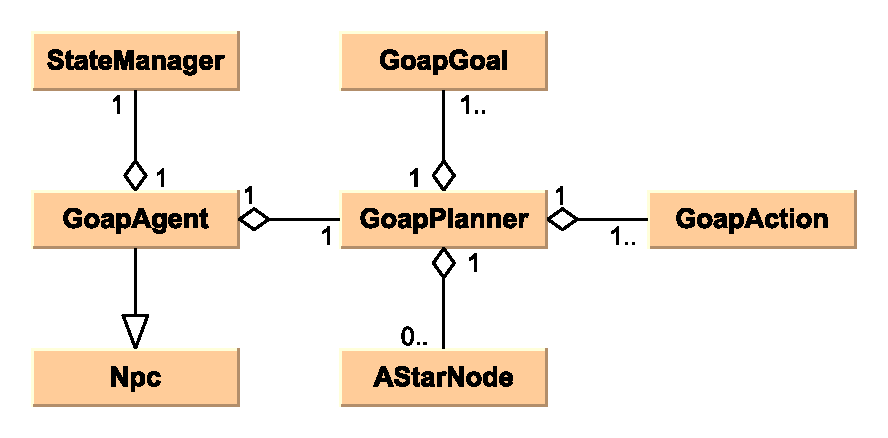
\includegraphics[width=0.8\textwidth, trim=20 20 20 20]{Implementation/goap arc.pdf}
	\captionsetup{justification=justified, format=plain}
  \caption{GOAP Architektur}
  \label{fig:GOAP Architektur}
\end{figure}







\subsection{\textit{GoapAgent}}
\label{chap:goapagent uml}

Die Abbildung \ref{fig:GoapAgent} stellt die Klasse \textit{GoapAgent}, mit ihren Klassenattribute und Methoden dar. Der \textit{goap\_planner} ist eine Referenz auf die Klasse \textit{GoapPlanner}, welcher die \textit{action\_se"=quence} des \textit{GoapAgent} bestimmt. Das Array \textit{action\_sequence} speichert Objekte vom Typ der Klasse \textit{GoapAction}. Sie stellt die ermittelte Aktions-Sequenz durch den A*-Algorithmus dar. Die Integer-Klassenvaraible \textit{current\_step} handelt als Indexzeiger, welcher auf die aktuell auszuführende Aktion des \textit{action\_sequence} verweist.


\begin{figure}[h]
  \centering
  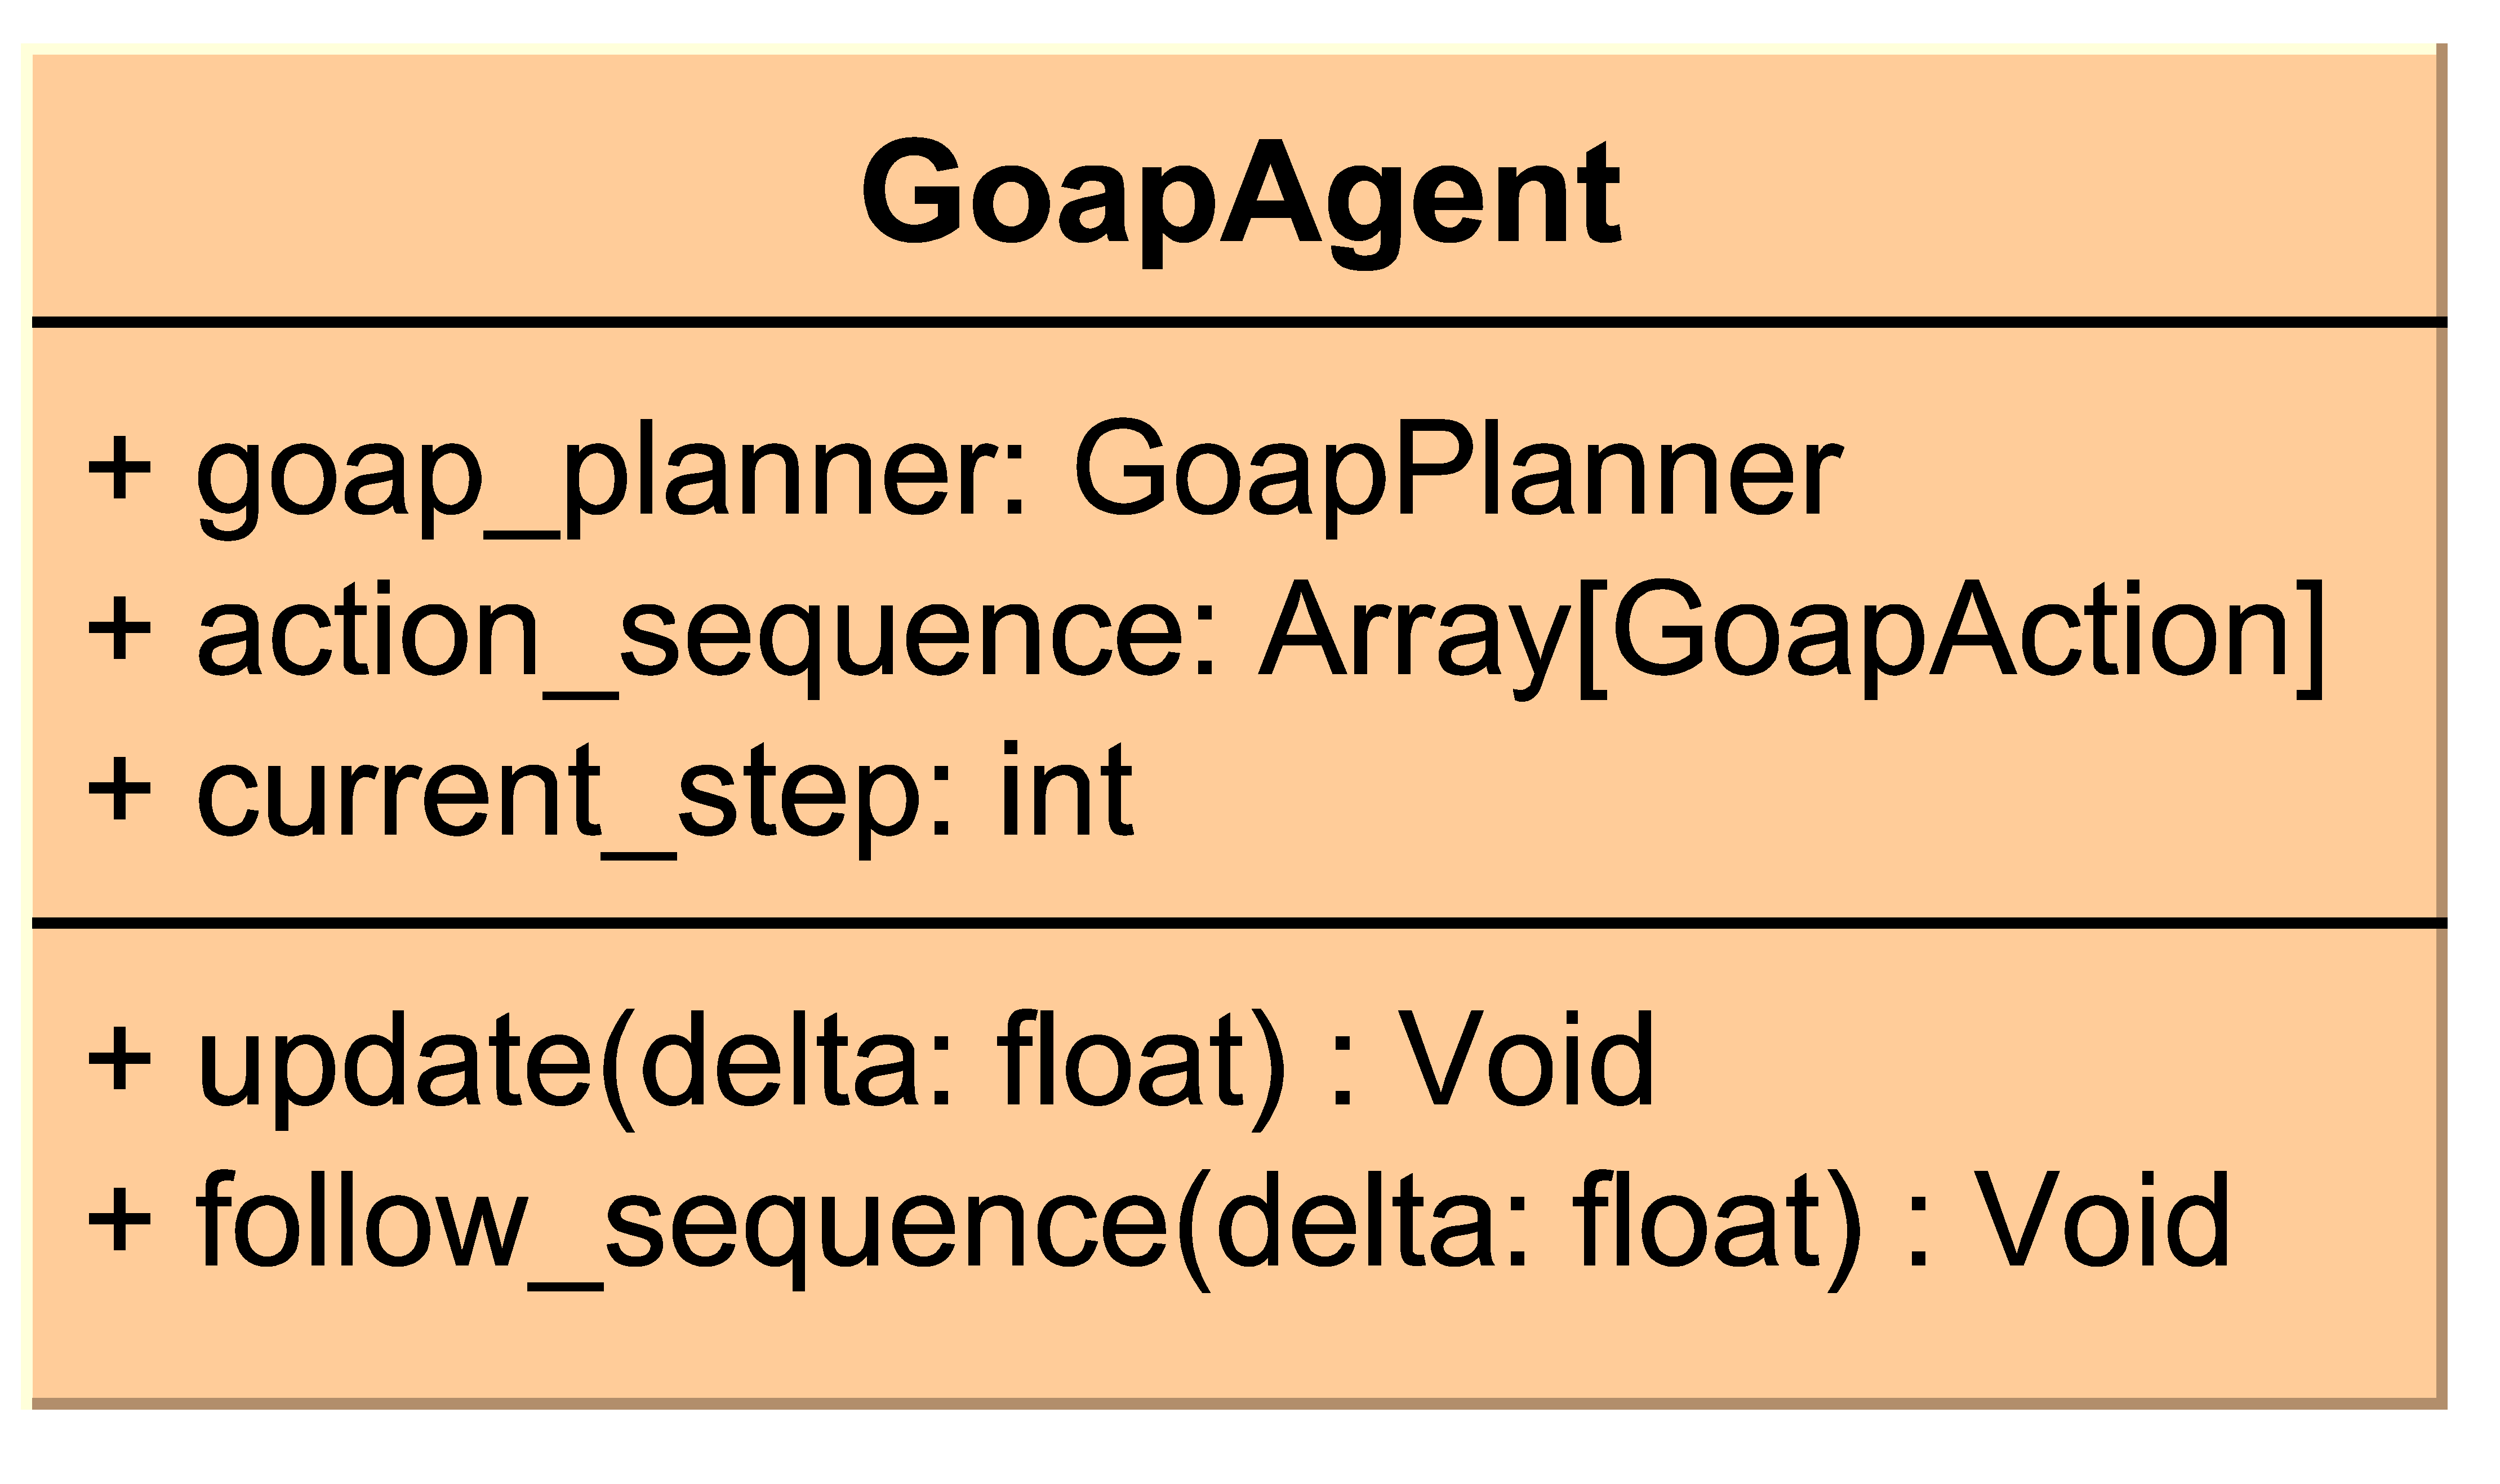
\includegraphics[width=0.5\textwidth]{Lösungskonzept/agent.pdf}
	\captionsetup{justification=justified, format=plain}
  \caption{GoapAgent}
  \label{fig:GoapAgent}
\end{figure}

Die update Methode (Pseudocode \ref{lst:pseudo update}) ruft Methoden der Klassen und Komponenten innerhalb des NPC auf. Sie wird wiederum durch eine \textit{\_process} Funktion jedes \textit{Frame} aufgerufen, um Komponenten \textit{GoapAgent} und und Abfragen nach \textit{actions\_sequence} auszuführen. Der Parameter \textit{delta} repräsentiert die Zeit seit dem letzten \textit{Frame} und könnte an andere Methoden übergeben werden. Wurde eine neue \textit{action\_sequence} vom \textit{goap\_planner} gefunden, so wird die Objektvariable \textit{current\_step} auf $0$ zurückgesetzt und die neue \textit{action\_sequence} aus dem \textit{goap\_planner} abgerufen. Die \textit{action\_sequence} wird darauf durch die Methode \textit{follow\_sequence} ausgeführt.

\"{U}ber die Methode \textit{follow\_sequence} geschieht die eigentliche Ausführung der Aktionen aus der \textit{action\_sequence}. Sollte \textit{action\_sequence} ungültig sein, so wird eine neue \textit{action\_sequence} durch \textit{goap\_planner.set\_create\_sequence(WAHR)} angefordert. Ansonsten wird mithilfe des \textit{current\_step} Index die jeweilige Aktion über ihre \textit{GoapAction} \textit{update} Methode ausgeführt. Bei erfolgreicher Ausführung der Aktion wird der \textit{current\_step} inkrementiert, um auf die nächste Aktion der \textit{action\_seqeunce} zuzugreifen.


\begin{lstlisting}[language=Pseudo, caption={update Methode des GoapAgent}, mathescape=true, label={lst:pseudo update}]
FUNKTION update(delta) $\rightarrow$ void
    WENN goap_planner.update() $\rightarrow$ neue action_sequence gefunden DANN
        current_step $\leftarrow$ 0
        action_sequence $\leftarrow$ goap_planner.get_current_sequence()
    ENDE WENN
    follow_sequence(delta)
ENDE update()

FUNKTION follow_sequence(delta) $\rightarrow$ void
	WENN action_sequence leer ODER action_sequence durchgegangen ODER action_sequence[current_step] DANN
		goap_planner.set_create_sequence(WAHR)
		ENDE follow_sequence()
	ENDE WENN
	WENN action_sequence[current_step].update(delta) ausgeführt DANN
		current_step um 1 erhöhen
	ENDE WENN
ENDE follow_sequence()
\end{lstlisting}














\subsection{\textit{GoapPlanner}}
\label{chap:goapplanner uml}


\begin{figure}[h]
  \centering
  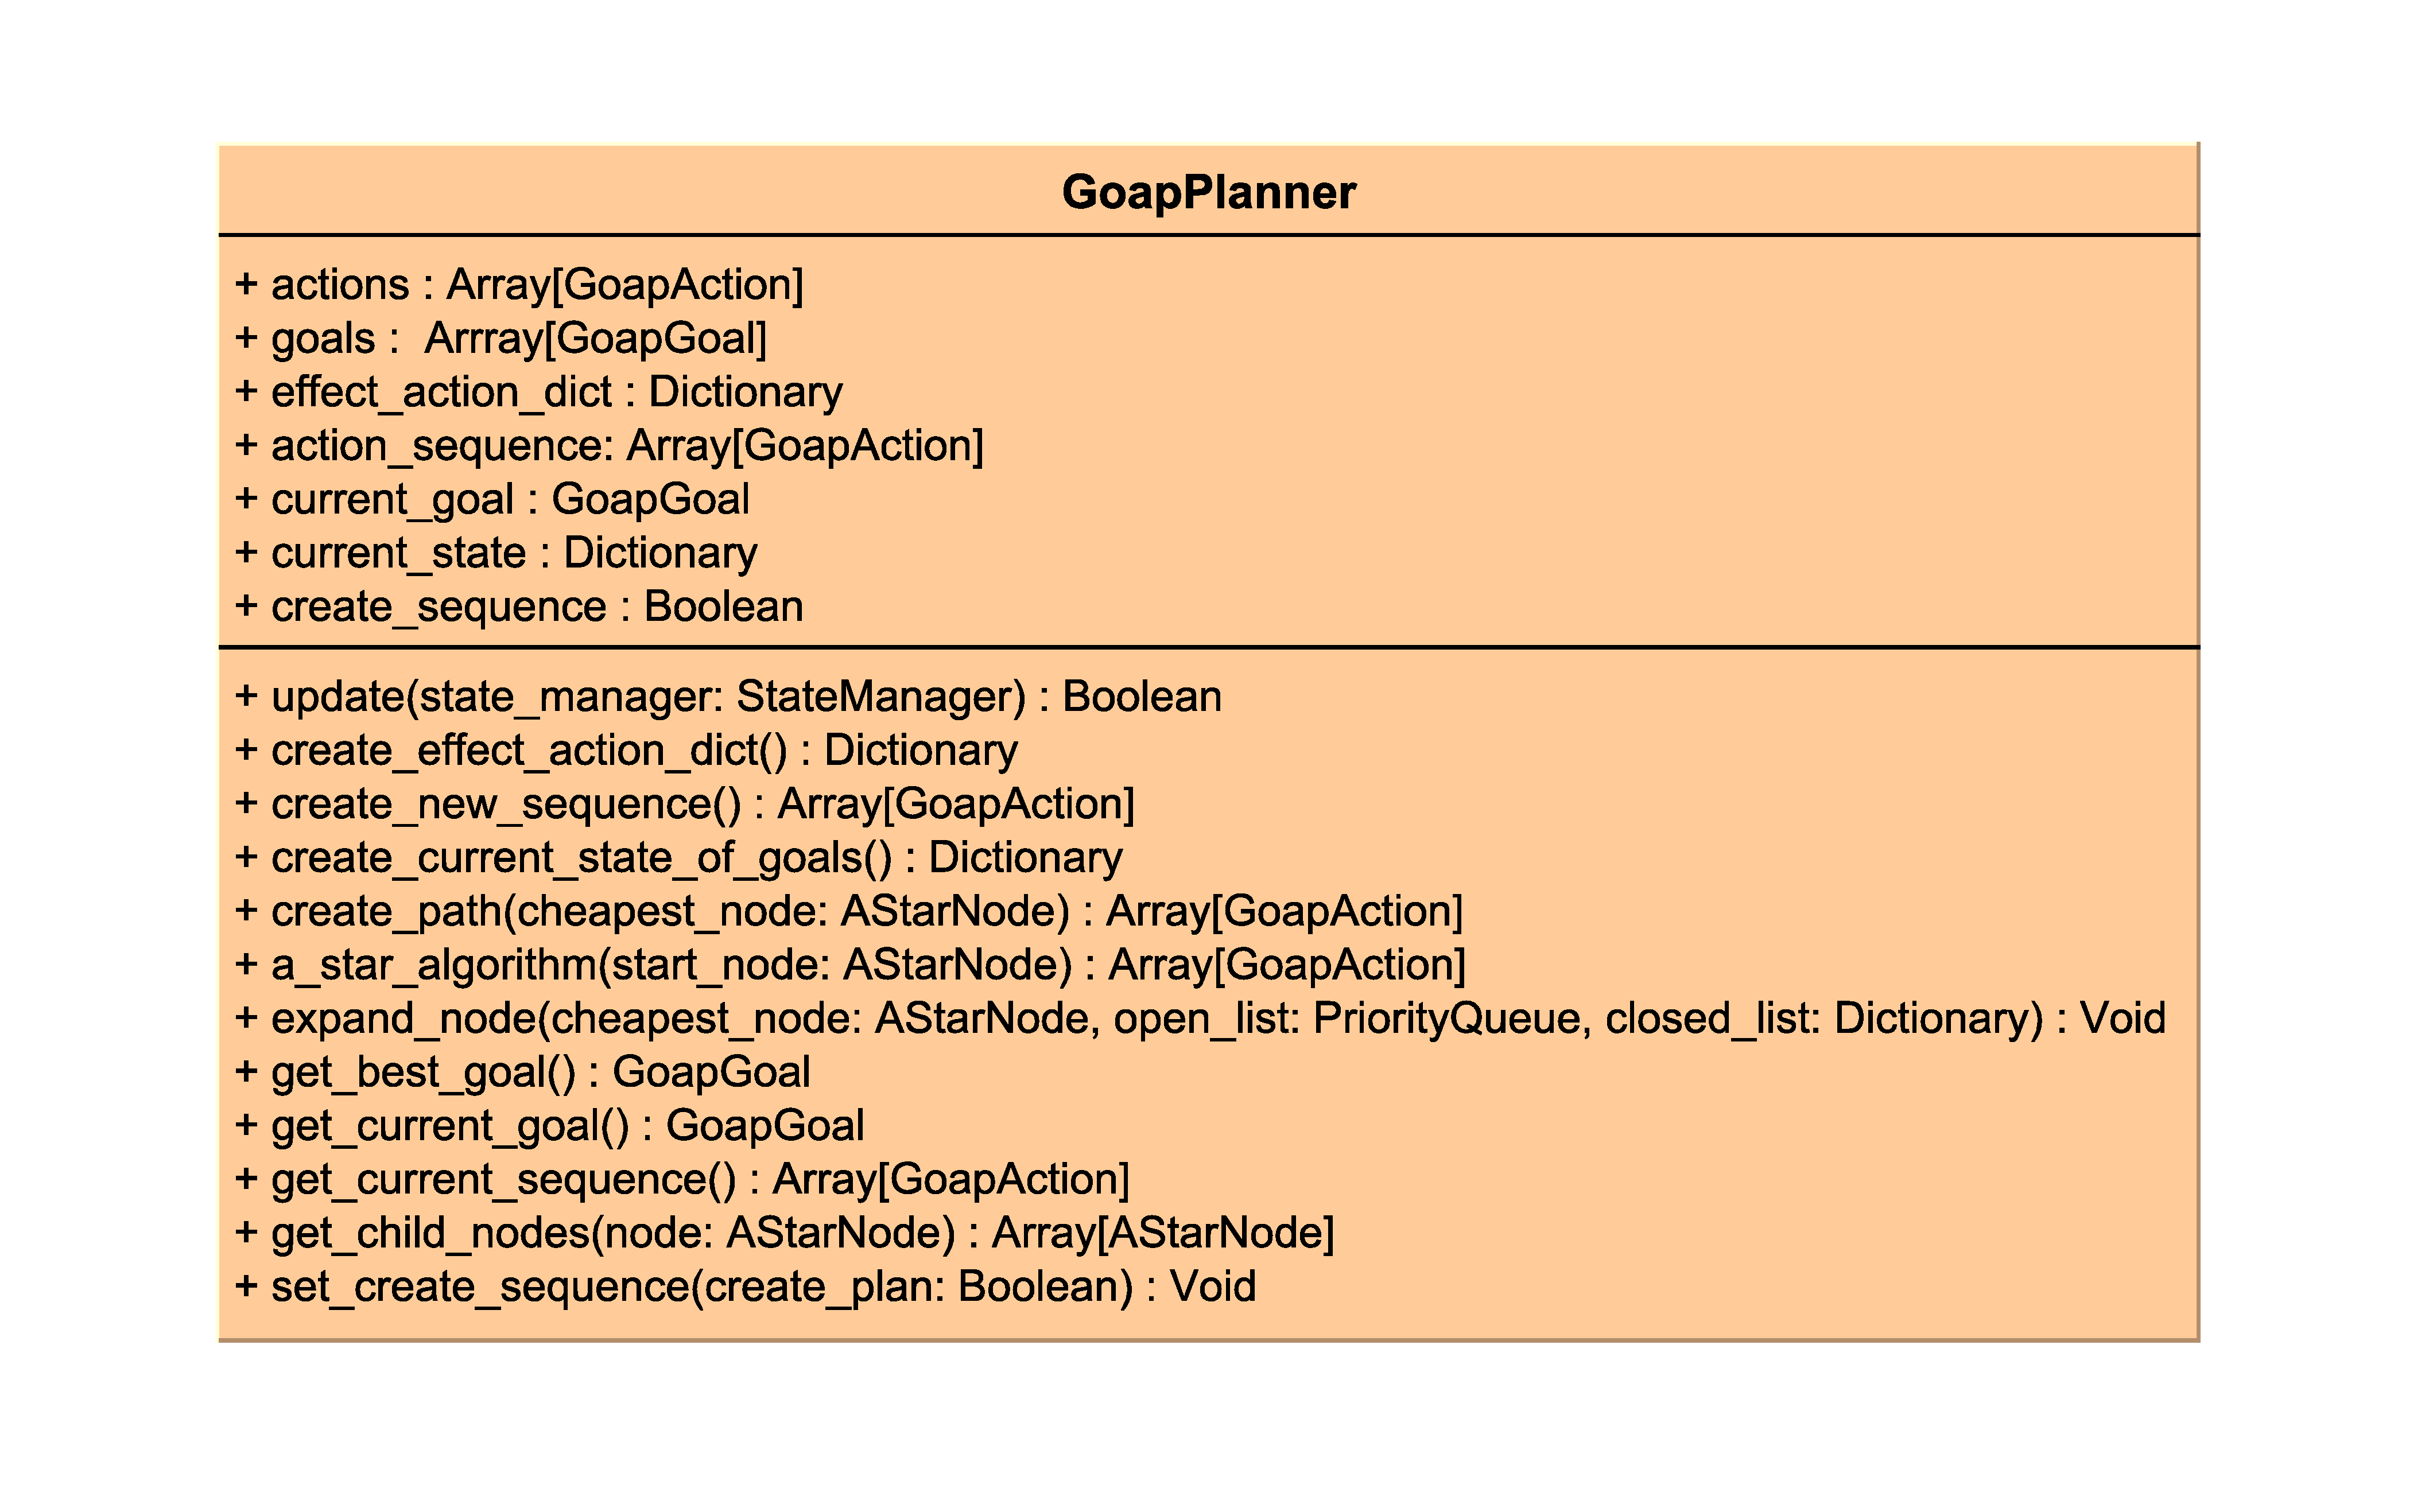
\includegraphics[width=\textwidth, trim=20 20 20 20]{Lösungskonzept/planner.pdf}
	\captionsetup{justification=justified, format=plain}
  \caption{GoapPlanner}
  \label{fig:goapplanner uml}
\end{figure}

Die Abbildung \ref{fig:goapplanner uml} zeigt den Aufbau des \textit{GoapPlanner}. Der \textit{GoapPlanner} arbeitet mit Zielen und Aktionen, welche durch die Arrays \textit{actions} und \textit{goals} gegeben werden. Das \textit{current\_state} Dictionary speichert den derzeitigen Zustand des \textit{GoapAgent}. Die Initialisierung des \textit{current\_state} findet über den \textit{state\_manager} Parameter statt, welcher über die \textit{update} Methode übergeben wird. Das \textit{create\_sequence} Attribut informiert den \textit{GoapPlanner} darüber, ob eine neue \textit{action\_sequence} generiert werden soll. 

Das \textit{effect\_action\_dict} Dictionary speichert alle möglichen Effekte als \textit{Schlüssel} und die zugehörigen \textit{GoapActions} als Werte, die diese Effekte herbeiführen. Sie setzt die Tabelle aus dem GOAP Grundlagenkapitel \ref{tab:aktions tabelle} um. Ähnlich wie im Goap-Beispiel werden gezielt \textit{GoapActions} gesucht, die bestimmte Effekte bewirken. Die Verwendung eines Dictionaries ermöglicht dabei schnellere Zugriffszeiten im Vergleich zu einer Array-basierten Suche.

% update
Die Methode \textit{update} des \textit{GoapPlanner} (Pseudocode \ref{lst:pseudo planner update}) wird über die \textit{update}-Methode des \textit{GoapAgent} aufgerufen. Sie bestimmt das aktuelle Ziel (\textit{current\_goal}) und die zugehörige Aktionssequenz (\textit{action\_sequence}). Die Auswahl des besten Ziels erfolgt über die Methode \textit{get\_best\_goal}. Falls sich das Ziel während der Laufzeit ändert oder \textit{create\_sequence} auf \textit{true} gesetzt ist, wird \textit{create_new\_sequence} eine neue Aktionssequenz generieren. Dazu wird ein Wurzelknoten des Typs \textit{AStarNode} erstellt, der an die \textit{a\_star\_algorithm} Methode übergeben wird. Ein \textit{AStarNode} (Klasse \ref{fig:AStarNode}) wird durch den Godot Konstruktor \_init instanziiert und besitzt die Eigenschaften eines Suchbaum-Knoten (Kapitel \ref{chap:knoten eines suchbaums}).

\begin{lstlisting}[language=Pseudo, caption={update Methode des GoapAgent}, mathescape=true, label={lst:pseudo planner update}]
FUNKTION update(state_manager: StateManager) $\rightarrow$ bool
    current_state $\leftarrow$ state_manager.get_current_state()
    new_goal $\leftarrow$ get_best_goal()
    WENN current_goal NICHT = new_goal ODER create_sequence WAHR IST DANN
        current_goal $\leftarrow$ new_goal
        action_sequence $\leftarrow$ create_new_sequence()
        root_node Speicher freigeben
        ZURÜCKGEBEN WAHR
    ENDE WENN
    ZURÜCKGEBEN FALSCH
ENDE FUNKTION
\end{lstlisting}

\begin{figure}[h]
  \centering
  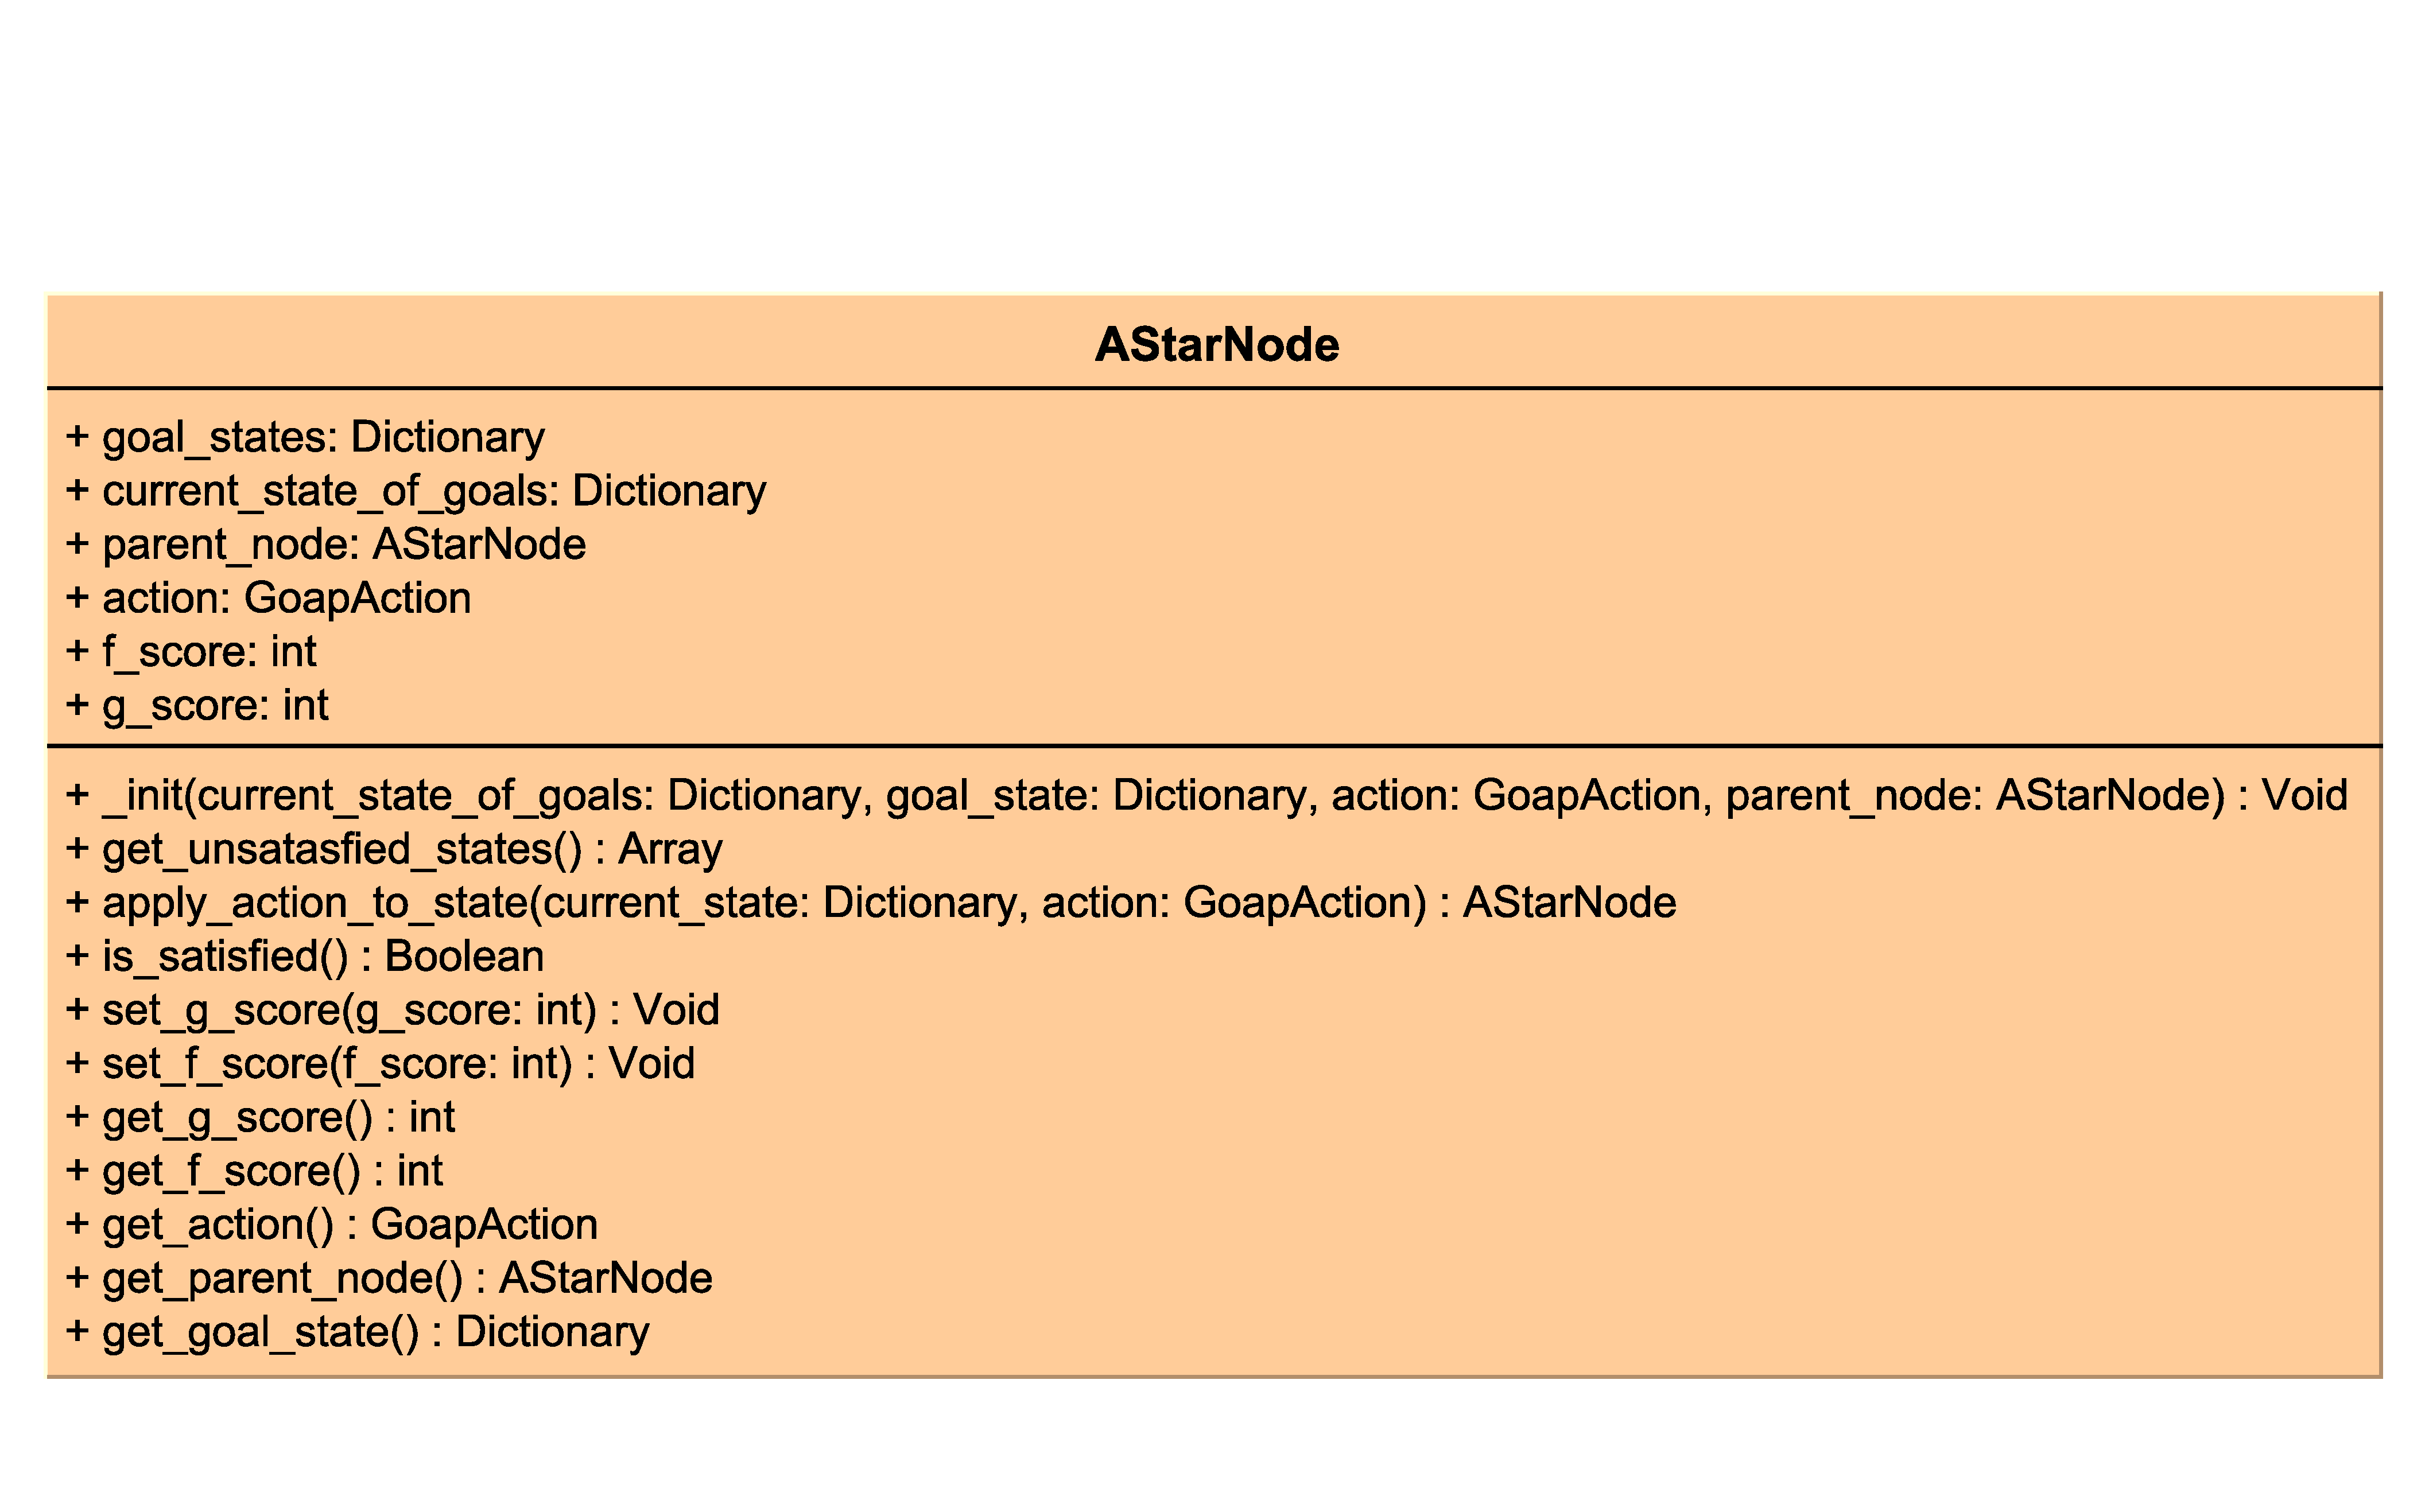
\includegraphics[width=0.9\textwidth, trim=20 20 20 20]{Lösungskonzept/astarnode.pdf}
	\captionsetup{justification=justified, format=plain}
  \caption{AStarNode}
  \label{fig:AStarNode}
\end{figure}

Die \textit{a\_star\_algorithm}-Methode (Pseudocode \ref{lst:pseudo astar}) sucht gemäß den Regeln der Bestensuche (Kapitel \ref{lst:pseudo bestensuche}) als A*-Algorithmus nach dem optimalen Pfad.

Darin speichert die \textit{open\_list} Knoten, deren Zustände noch nicht erfüllt sind. Sie wird als Prioritätswarteschlange implementiert und enthält \textit{AStarNode}-Knoten, die nach ihren geschätzten Gesamtkosten $f(n)$ sortiert sind. Da Godot 4.3 keine native Prioritäts-Warteschlange bietet, muss diese manuell umgesetzt werden. Ein einfaches Array wäre möglich, würde aber die Zugriffszeiten erhöhen. Die \textit{closed\_list} ist ein Dictionary bereits besuchter \textit{AStarNodes}, und vermeidet Mehrfachbesuche. 

Zunächst wird der \textit{root\_node} in die \textit{open\_list} eingefügt. Anschließend beginnt eine Schleife, die so lange läuft, wie noch Knoten in der \textit{open\_list} vorhanden sind. In jeder Iteration wird der Knoten mit den geringsten Kosten aus der \textit{open\_list} entnommen und als \textit{expanded\_node} gesetzt. Sollte dieser Knoten bereits alle Bedingungen erfüllen, wird die Methode \textit{create\_path} aufgerufen, um die optimale Aktionssequenz zu rekonstruieren, und das Ergebnis wird zurückgegeben. Falls der \textit{expanded\_node} noch zu erfüllende Zustände besitzt, wird er in die \textit{closed\_list} aufgenommen und an die Methode \textit{expand\_node} weitergegeben. Falls die \textit{open\_list} nach Abschluss der Schleife leer ist, wird eine leere Aktionssequenz zurückgegeben, da kein gültiger Pfad gefunden wurde.

Die Methode \textit{expand\_node} ist für die Erweiterung des aktuell expandierten Knotens verantwortlich. Sie iteriert über alle möglichen Kindknoten (\textit{child\_nodes}), die sich aus den möglichen Aktionen ergeben. Falls ein Kindknoten bereits in der \textit{closed\_list} enthalten ist, wird dieser übersprungen. Andernfalls wird die Pfadkostenfunktion $g(n)$ des Kindknotens berechnet, indem die Kosten der aktuellen Aktion zu den Kosten des Vorgängerknotens addiert werden. Anschließend wird überprüft, ob der Kindknoten bereits in der \textit{open\_list} existiert und ob der neue Pfad kostenintensiver ist als ein zuvor gespeicherter Pfad zu diesem Knoten. Ist dies der Fall, wird die Iteration für diesen Knoten abgebrochen. Falls der Knoten weiterhin in Betracht gezogen wird, wird die geschätzte Heuristik $h(n)$ berechnet, indem die Anzahl unerfüllter Zustände ermittelt wird. Die Gesamtkosten $f(n)$ setzen sich aus der Summe von $g(n)$ und $h(n)$ zusammen. Anschließend werden die berechneten Werte im Kindknoten gespeichert, und dieser wird in die \textit{open\_list} eingefügt, um in einer späteren Iteration betrachtet zu werden.

\begin{lstlisting}[language=Pseudo, caption={a\_star\_algorithm Methode}, mathescape=true, label={lst:pseudo astar}]
FUNKTION a_star_algorithm(root_node) $\rightarrow$ action_sequence
	open_list $\leftarrow$ PriorityQueue
	closed_list $\leftarrow$ Dictionary
	open_list.push(root_node)
	SOLANGE open_list NICHT leer
		expanded_node $\leftarrow$ open_list.pop()
		WENN expanded_node.is_satisfied() DANN
			open_list Speicher freigeben
			ZURÜCKGEBEN $\rightarrow$ create_path(expanded_node)
		ENDE WENN
		expanded_node in closed_list hinzufügen
		expand_node(expanded_node, open_list, closed_list)
	ENDE SOLANGE
	open_list Speicher freigeben
	ZURÜCKGEBEN $\rightarrow$ []
ENDE a_star_algorithm()

FUNKTION expand_node(expanded_node, open_list, closed_list) $\rightarrow$ void
	FÜR JEDES child_node IN get_child_nodes(expanded_node)
		WENN child_node IN closed_list DANN
			FORTSETZEN
		ENDE WENN
		child_node_g_cost $\leftarrow$ expanded_node.get_g_score() + child_node.get_action().get_cost()
		WENN open_list.has(child_node) UND child_node_g_cost $\geq$ child_node.get_g_score() DANN
			FORTSETZEN
		ENDE WENN
		child_node_h_cost $\leftarrow$ child_node.get_unsatisfied_states().size()
		child_node_f_cost $\leftarrow$ child_node_g_cost + child_node_h_cost
		child_node.set_g_cost(child_node_g_cost)
		child_node.set_f_cost(child_node_f_cost)
		open_list.push(child_node)
	ENDE FÜR
ENDE expand_node()
\end{lstlisting}





\subsection{GoapGoal}
\label{chap:goapgoal uml}

Die \textit{GoapGoal} Klasse wird in der Abbildung \ref{fig:GoapGoal} dargestellt. Die Eigenschaften eines Goap-Zieles, also die Priorität und die Gültigkeit werden aus dem \textit{StateManager} durch die Methoden \textit{get\_priority} und \textit{is\_valid} dynamisch abgeleitet. Der \textit{GoapPlanner} benötigt die Gültigkeit und Priorität, um in folge dessen das Ziel auszuwählen. Ein Ziel wird erst dann berücksichtigt, wenn es durch die Methode \textit{is\_valid} als gültig bestätigt wurde. Anschlie\ss{}end kann dessen Priorität mithilfe von \textit{get\_priority} ermittelt werden. \"{U}ber die Methode \textit{get\_desired\_state} werden die Zielzustände aufgerufen, welche der \textit{GoapPlanner} zur Suche der \textit{action\_sequence} benötigt. Die Methode \textit{get\_goal\_name} gibt den Klassennamen des GoapGoal zurück, welche von Debug Methoden genutzt werden kann.

\begin{figure}[t]
  \centering
  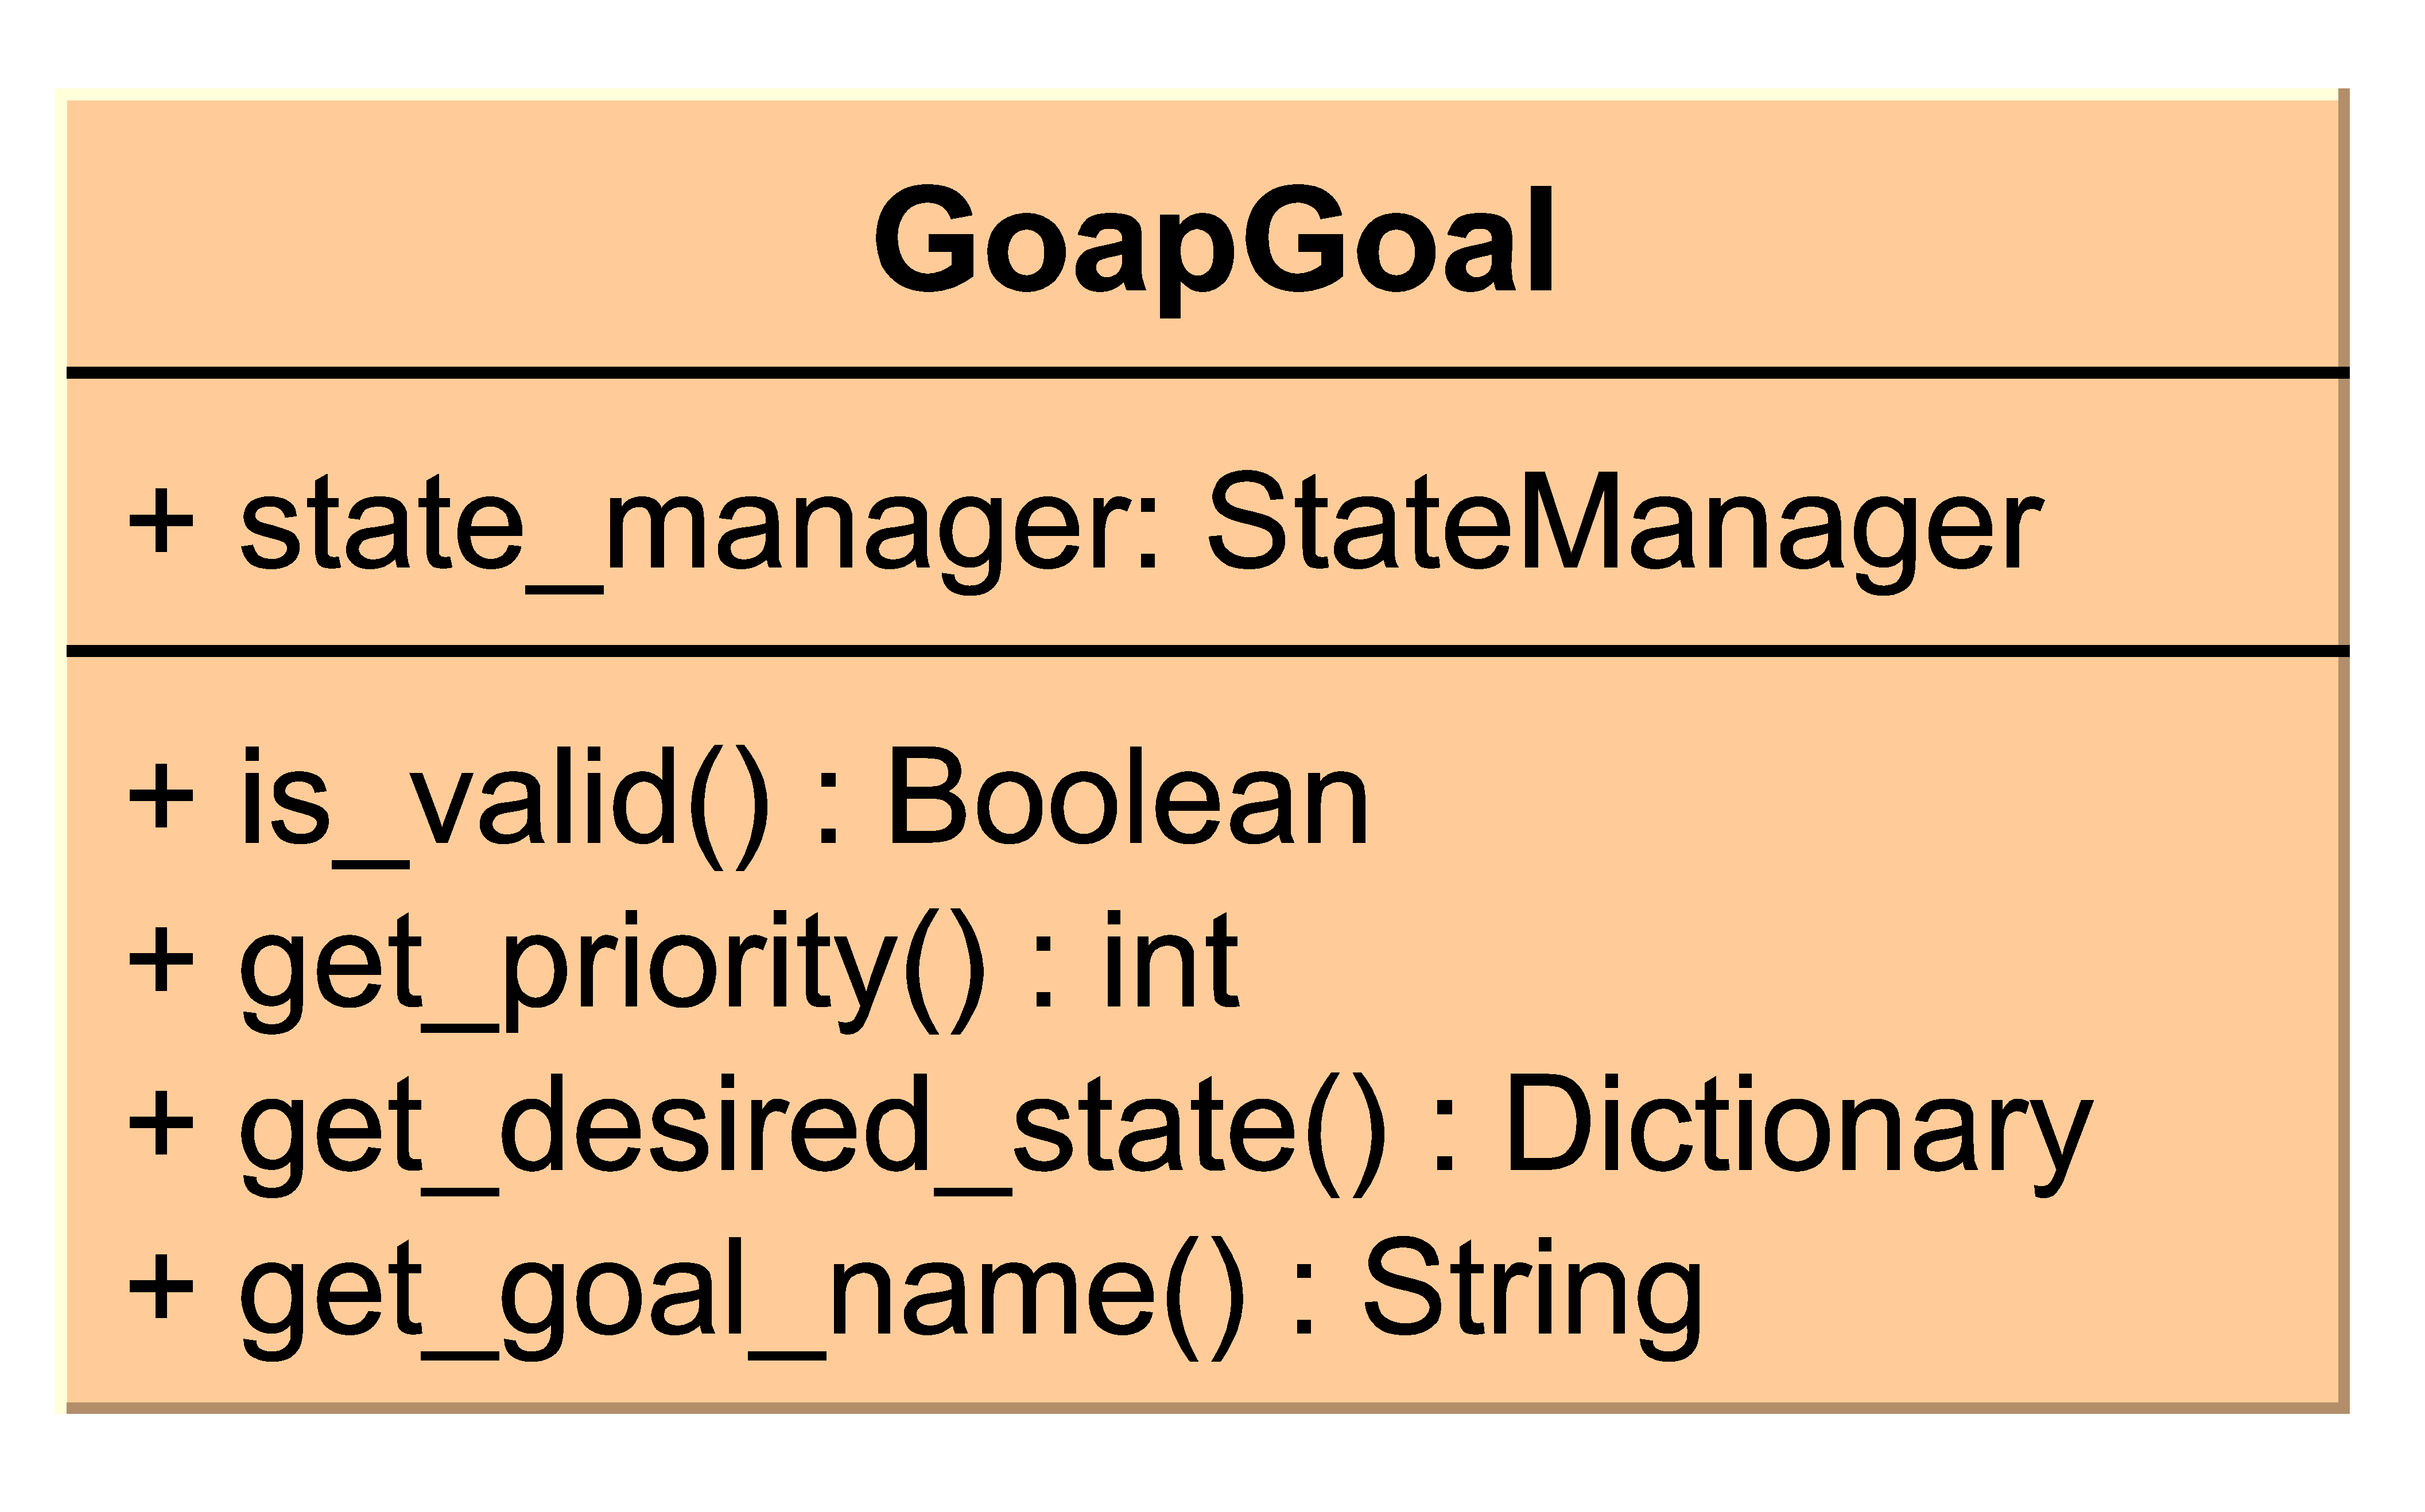
\includegraphics[width=0.5\textwidth, trim=20 20 20 20]{Lösungskonzept/goal.pdf}
	\captionsetup{justification=justified, format=plain}
  \caption{GoapGoal}
  \label{fig:GoapGoal}
\end{figure}







\subsection{GoapAction}
\label{chap:goapaction uml}

Die \textit{GoapAction} Klasse wird in der Abbildung \ref{fig:GoapAction} dargestellt. Eine \textit{GoapAction} gibt seine Kosten und Gültigkeit wieder. Dabei werden die Kosten $g(n)$ mittels den Klassenattributen \textit{character\_body} und \textit{state\_manager} über die \textit{get\_cost} Methode dynamisch berechnet.

Die Gültigkeit einer Aktion soll die Durchführbarkeit wiedergeben. Der \textit{GoapPlanner} wählt nur Aktionen aus, welche im derzeitigen Zustand des NPC durchführbar sind. Die Gültigkeit der Aktionen wird auch vor der Ausführung der update Methode jeweiligen Aktion durch den \textit{GoapAgent} geprüft, da die Aktion zu einer Zeit ausgeführt werden kann in der sich der Zustand des NPC wieder ändern kann und somit auch die Gültigkeit. Für die Rückgabe der Gültigkeit ist die is\_valid Methode zuständig.

Eine get\_preconditions Methode gibt die vorausgesetzten Zustände zurück, welche von anderen Aktionen erfüllt werden müssten. Ob eine Aktion einen Zustand erfüllen kann, hängt von der get\_effects Methode ab, welche ein \textit{Dictionary} mit dem Zustand und dessen Wert zurückgibt. Stimmt der Wert des Zustands mit dem Zielzustand überein, dann erfüllt die Aktion den Zustand.

Die update Methode leitet die eigentliche Ausführung der Aktion ein und wird über den \textit{GoapAgent} gestartet. Die Hoffnung dabei ist, dass die Aktion den erwünschten Wert des Effekts umsetzt. Aufgrund der nicht-deterministischen Natur der Spielwelt kann es jedoch vorkommen, dass der angestrebte Effekt nicht erreicht wird. Wird der Effekt nicht erreicht, so wird eine neue Sequenz angefordert oder das Ziel ändert sich bis dahin. Die Ausführung der Aktion wird dabei über Komponenten der Klasse Npc umgesetzt. Die Methode get\_action\_name gibt den Klassennamen der \textit{GoapAction} zurück.

\begin{figure}[h]
  \centering
  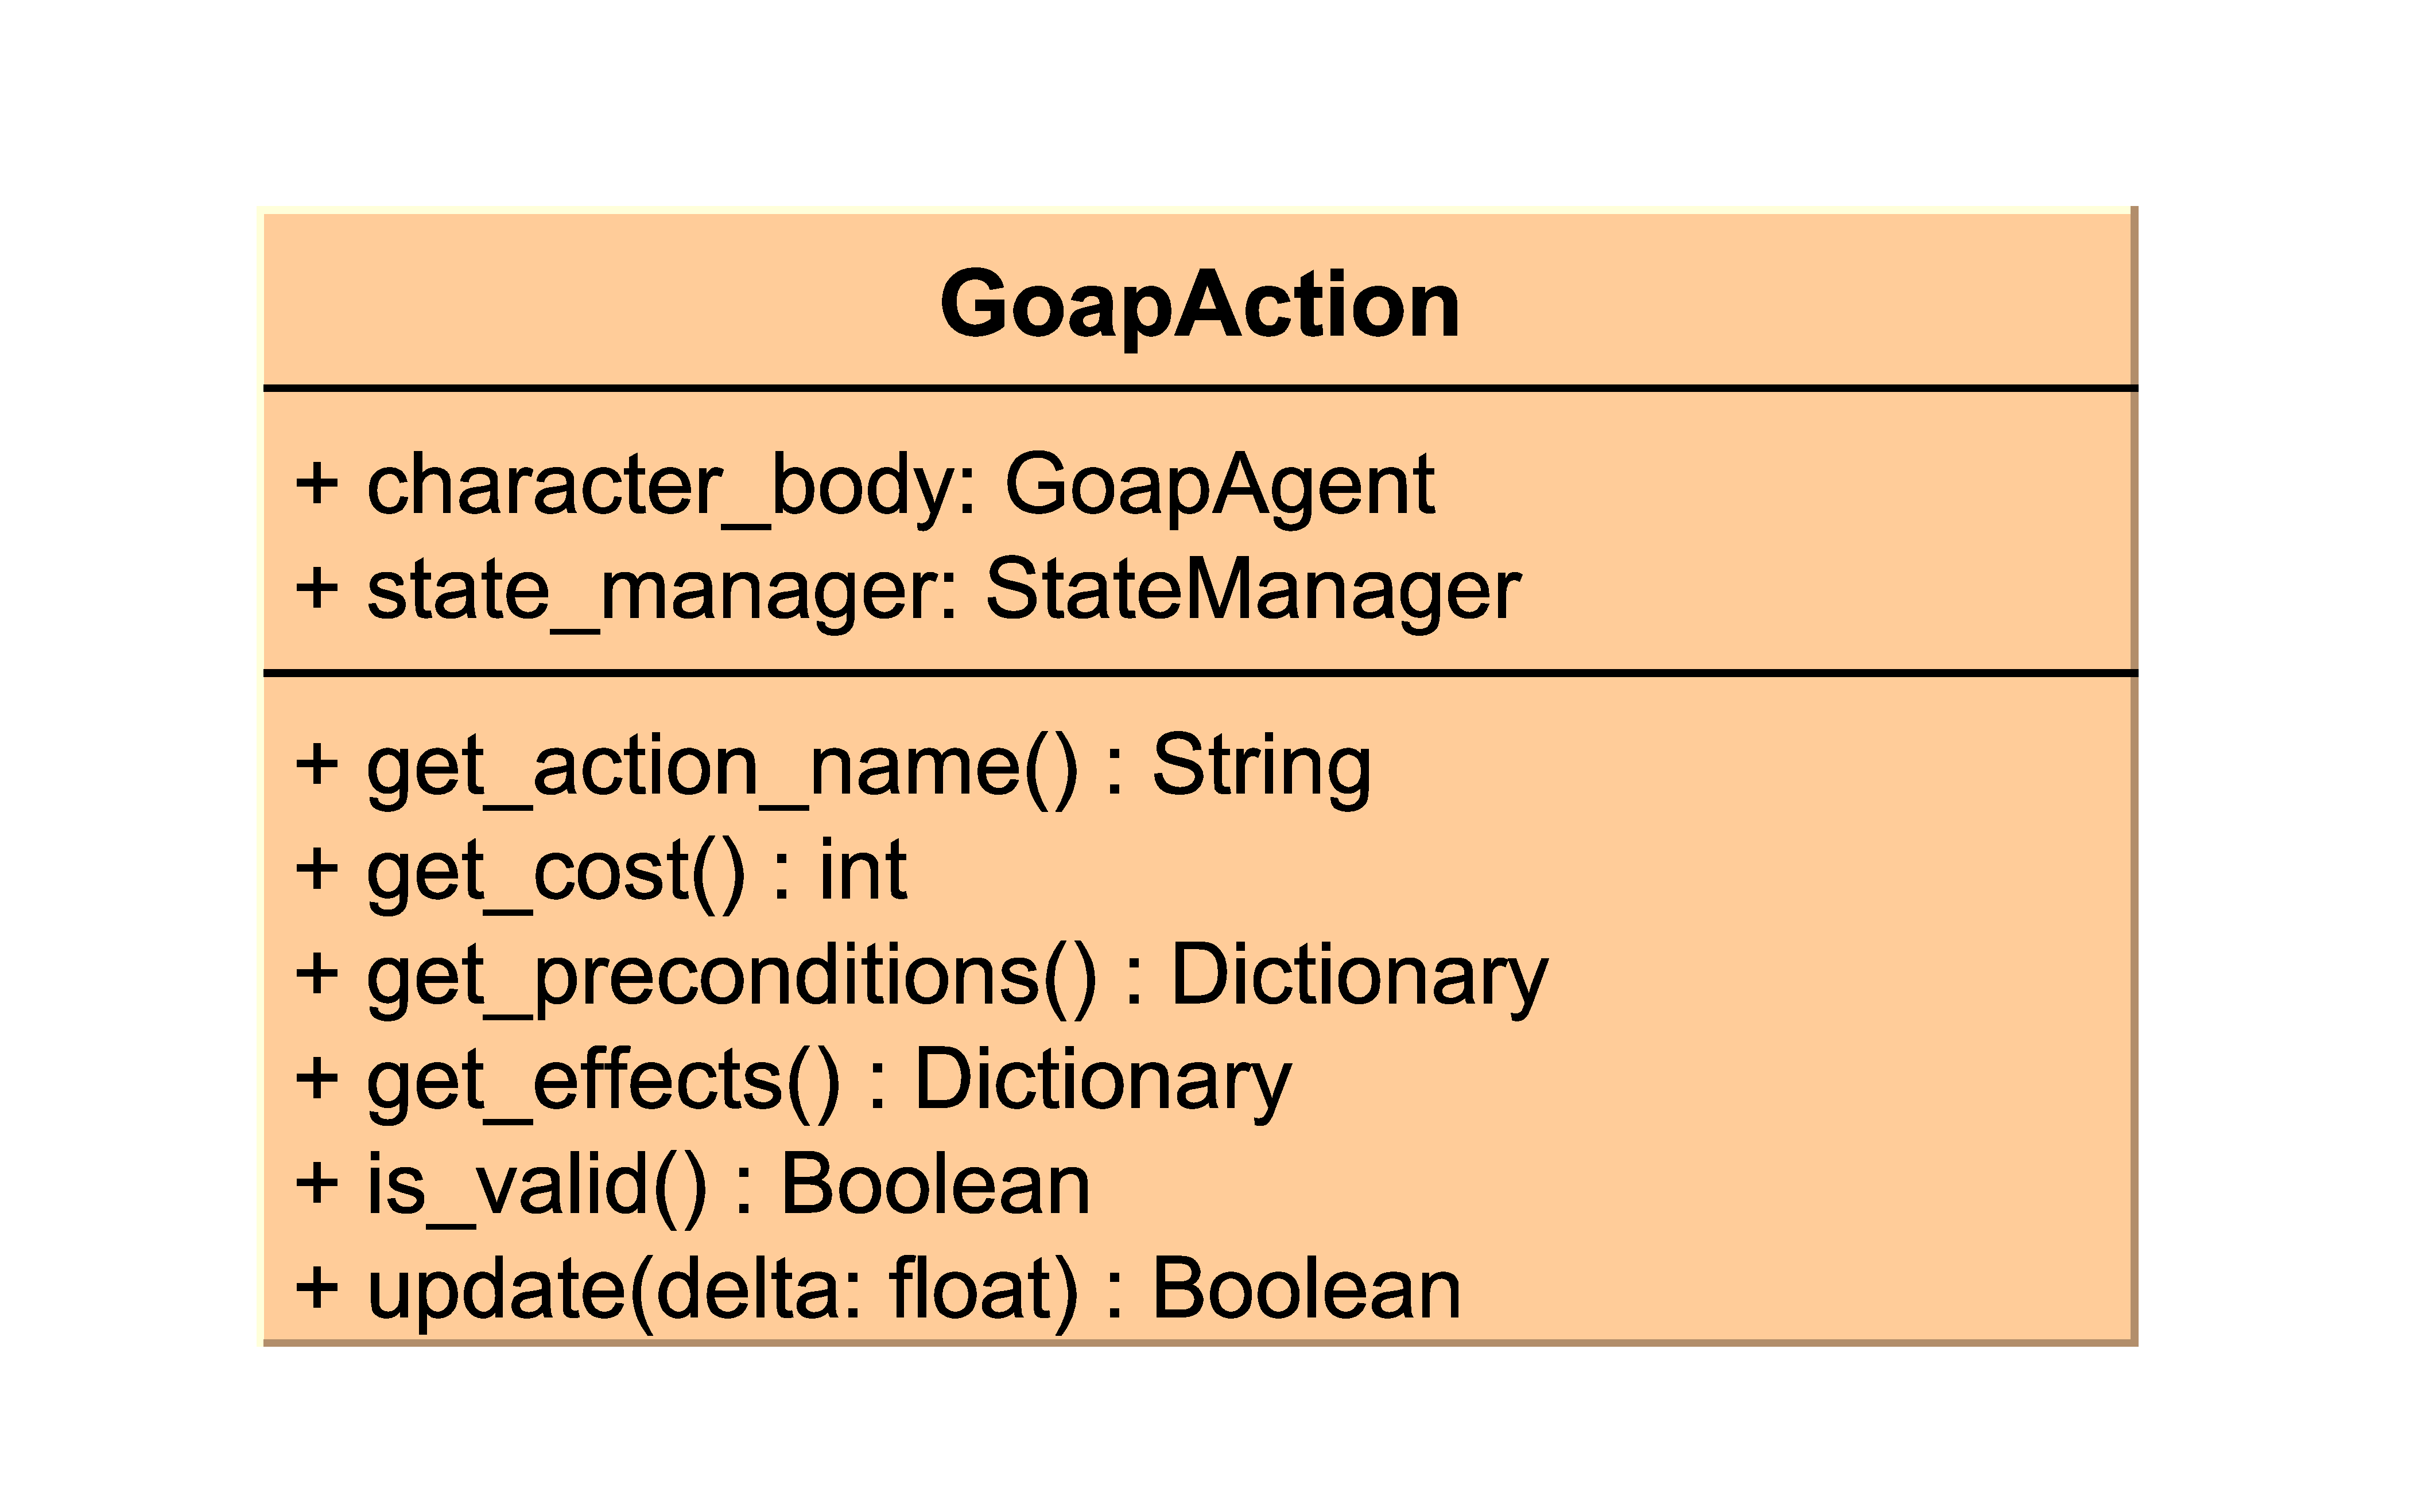
\includegraphics[width=0.7\textwidth, trim=20 20 20 20]{Lösungskonzept/action.pdf}
	\captionsetup{justification=justified, format=plain}
  \caption{GoapAction}
  \label{fig:GoapAction}
\end{figure}








\section{Umsetzung des Szenario}
\label{chap:implementierung szenario}

Die Benchmarks benötigen eine Umgebung auf der die NPCs mit ihren jeweiligen Entscheidungssystemen getestet werden. Zu diesem Zweck agieren die NPCs\ref{} in einer 2D kartierbaren Spielwelt, die in der Abbildung \ref{} dargestellt wird. Die NPC-Klassen unterscheiden sich in ihren Entscheidungssystemen, die Komponenten, die für eine Ausführung einer Aktion benötigt werden bleiben für alle NPC Klassen identisch und werden mit der Oberklasse Npc vererbt. Bei den Komponenten handelt es sich um: Vision-, Health-, Hit-, Melee-, Shoot-, Neighbor-, Move, LookAt-, Patrol-, Cover-, Vision- und PlayerBlock-Component. Sie ändern dabei die Zustände des StateManger, die in der GOAP Architektur erläutert wird\ref{}.

\begin{figure}[h]
  \centering
  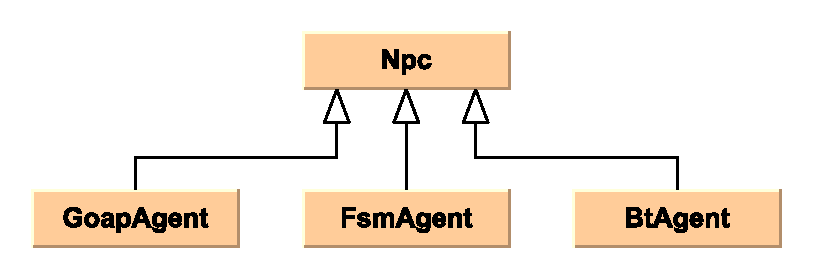
\includegraphics[width=0.7\textwidth, trim=20 20 20 20]{Implementation/npc class.pdf}
	\captionsetup{justification=justified, format=plain}
  \caption{Vererbung der Npc Klasse}
  \label{fig:npc class}
\end{figure}

\begin{figure}[h]
  \centering
  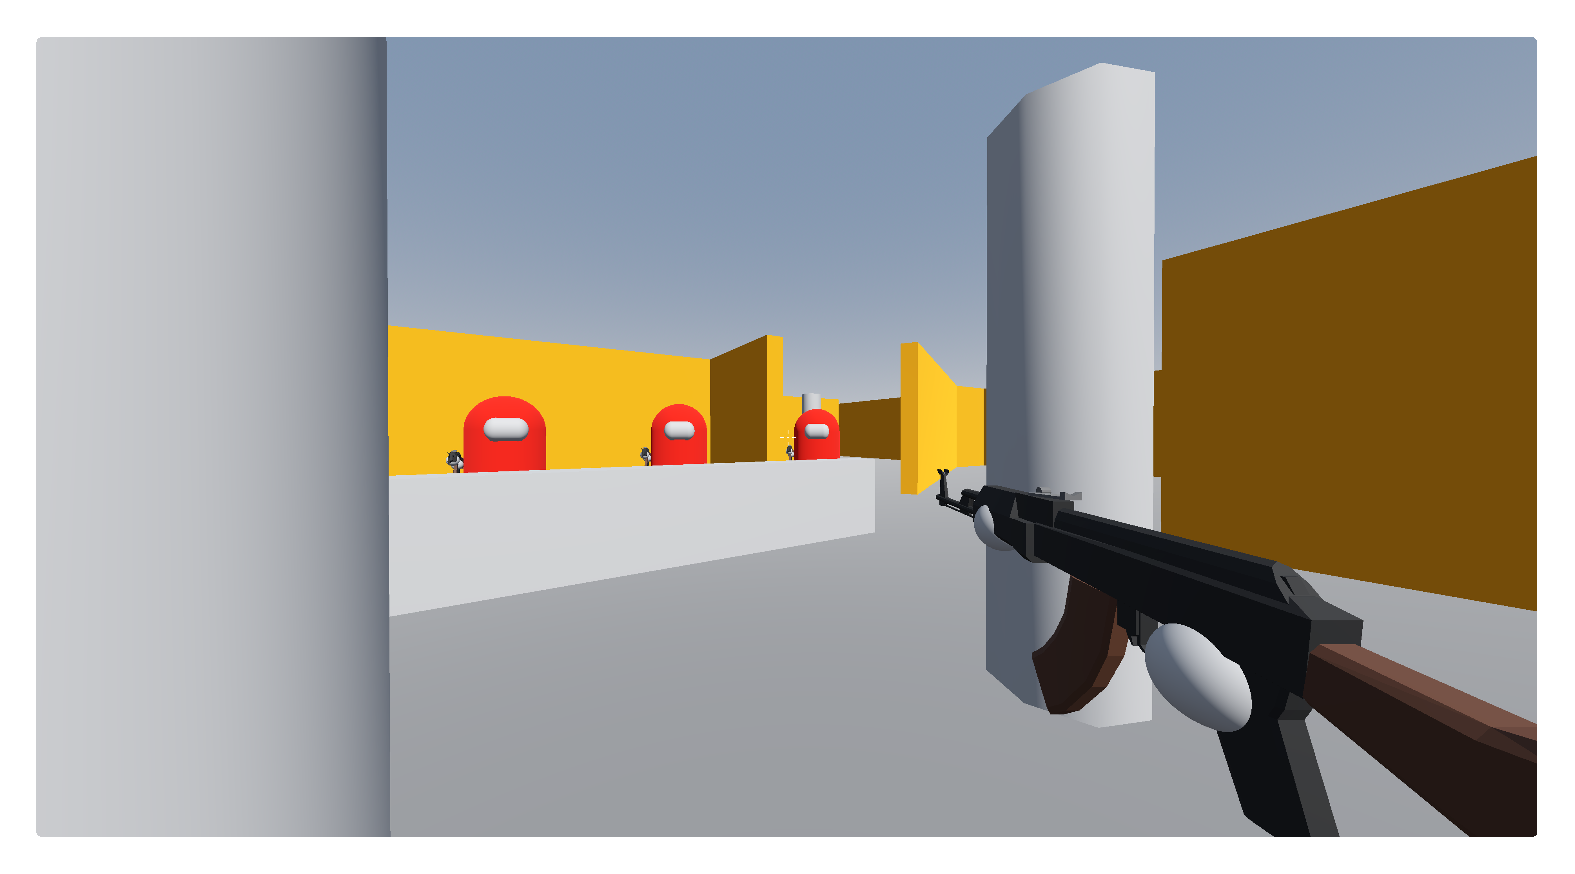
\includegraphics[width=0.7\textwidth, trim=20 20 20 20]{Implementation/ego shooter.pdf}
	\captionsetup{justification=justified, format=plain}
  \caption{Ego-Perspektive des Spieler und Spielwelt}
  \label{fig:ego shooter}
\end{figure}

Der Performance-Benchmark\ref{fig:bps benchmark}, speichert während der Ausführung die Häufigkeit der Bilder-Pro-Sekunde für die jeweilige Anzahl an NPCs im gesamten Szenario. Der Benchmark beginnt mit einem NPC und wächst kontinuierlich, wobei alle 30 Sekunden ein neuer NPC der jeweiligen Klasse in die Spielwelt instanziiert wird. Für jede NPC-Klasse wird der Benchmark dreimal ausgeführt. Abschlie\ss{}end wird aus den gesammelten Daten der durchschnittliche FPS-Wert für jede NPC-Anzahl berechnet.

Der Speicher-Benchmark\ref{fig:mem benchmark}, gibt den Speicherverbrauch des gesamten Szenario. Auch dieser Benchmark beginnt mit einem NPC und wächst kontinuierlich, wobei alle 10 Sekunden ein neuer NPC der jeweiligen Klasse in die Spielwelt instanziiert wird. Für jede NPC-Klasse wird der Benchmark einmal ausgeführt. Abschlie\ss{}end wird auch hier aus den gesammelten Daten der durchschnittliche Speicherverbrauch für jede NPC-Anzahl berechnet.
